\documentclass{article}

\usepackage{tabularx}

% NOTE: To put equations in their environment we need either `float` or
% `caption`.  We use float to put equations and other environments exactly
% where they appear in the code with the `H` placeholder, and for that we
% redefine the `equ` environment sort of twice, so this is a bit flaky but
% it works.
\usepackage{caption}
\DeclareCaptionType{equ}[][]
\captionsetup[equ]{name=נוסחא}
\usepackage{float}
\floatstyle{plain}
% https://www.overleaf.com/learn/latex/Positioning_of_Figures
\newfloat{equ}{H}{eq}[section]
\floatname{equ}{נוסחא}

\DeclareCaptionType{graph}[][]
\captionsetup[graph]{name=גרף }

% to includegraphics
\usepackage{graphicx}

% to fix itemize lists:
% https://tex.stackexchange.com/a/53453/125609
\usepackage{enumitem}
\setlist[itemize,1]{label={\fontfamily{cmr}\fontencoding{T1}\selectfont\textbullet}}

% Links
\usepackage{hyperref}
\hypersetup{colorlinks = true,
	citecolor = gray,
	linkcolor = red,
	citecolor = green,
	filecolor = magenta,
	urlcolor = cyan
}

% To include plots by matplotlib
\usepackage{pgfplots}
\pgfplotsset{compat=newest}
% Note we use resizebox as explained here through out the document https://tex.stackexchange.com/a/582956/125609

% Language
\usepackage{polyglossia}
\setdefaultlanguage{hebrew}
\setotherlanguage{english}
\usepackage{hebrewcal}

% Fonts
\setmainfont{David CLM}
\setsansfont{Liberation Sans}
\setmonofont{Liberation Mono}
\newfontfamily\hebrewfont{David CLM}[Script=Hebrew]
\newfontfamily\hebrewfontsf{Liberation Serif}[Script=Hebrew]
\newfontfamily\hebrewfonttt{Liberation Mono}[Script=Hebrew]

\title{
שימוש באפקט
\textenglish{Hall}
למדידת פער אנרגטי בין רמות אנרגיה במוליך למחצה מסוג
\textenglish{n-Germanium}
}
\author{
שרה לחצר ודורון בכר \\
הפקולטה לפיזיקה, הטכניון - מכון טכנולוגי לישראל.
}
\date{\today}

\begin{document}
\maketitle

\begin{abstract}
% TODO
\end{abstract}
\section{מבוא}
\subsection{אפקט הול}
אפקט הול הוא תופעה פיזיקלית בה נוצר מתח חשמלי בכיוון ניצב לכיוון זרימת זרם במוליך, כאשר מופעל על המוליך שדה מגנטי ניצב. 
השדה המגנטי יוצר כוח על נושאי המטען שכיוונו ניצב לכיוון הזרימה ולשדה המגנטי, כך תיווצר הצטברות מטען שלילי בקצה אחד של המוליך ומטען חיובי בקצה המנוגד שיוצרו שדה חשמלי במוליך.
 לבסוף, המערכת תגיע לשיווי משקל כאשר הכוח שיוצר השדה החשמלי יבטל את הכח שיוצר השדה המגנטי.
במצב זה, המתח הנמדד בניצב לזרם- מתח הול- נתון בנוסחא
\ref{equ:V_hall}.
\begin{equ}
$$V_H = \frac{IB}{ned}$$
\caption{מתח הול כתלות בזרם 
$I$,
 בשדה המגנטי
$B$,
בצפיפות נושאי המטען
$n$,
ובמרחק בין קצוות המוליך בכיוון של שדה הול
$d$.}
\label{equ:V_hall}
\end{equ}


\begin{equ}
$$R_H = \frac{1}{ne}$$
\caption{מקדם הול עבור נושא מטען יחיד}
\label{equ:R_hall}
\end{equ}

\subsection{מוליכים למחצה}
מוליכים למחצה הם חומרים מהטור הרביעי של הטבלה  המאופיינים ב-4 אלקטרוני ערכיות. כאשר החומר מסודר כגביש טהור, כל אטום בשריג הגבישי הוא בעל 4 שכנים איתם הוא נמצא בקשר קוולנטי, כך שלמעשה בכל המערכת אין אלקטרונים חופשיים להולכה. גביש כזה נקרא מוליך למחצה אינטרינזי.
על מנת להגדיל את ההולכה של המל"מ מבצעים אילוח
על ידי הוספה של חומרים מהעמודה החמישית או השלישית.
בעת הוספת חומרים מהעמודה החמישית נוספים אלקטרונים עודפים למערכת, ואילו בעת הוספת  חומרים מהעמודה השלישית נוצרים קשרים קוולנטיים בהם חסר אלקטרון.
מחסור בקשר הקוולנטי באלקטרון נקרא חור והוא מתנהג כמו נושא מטען חיובי.

במל"מ אינטרינזי בש.מ סה"כ ריכוז החורים קבוע וריכוז אלק' קבוע כי בממוצע על כל אלק' שעולה לפס
ההולכה ויוצר חור, יש אחד שיורד לרמת הערכיות וממלא חור.
כעת נקבל את אפקט הול עבור שני נושאי מטען ולכן נקבל נוסחא חדשה למקדם הול הנתונה בנוסחא
\ref{equ:R_hall_2_carriers}.
\begin{equ}
$$R_H = \frac{\mu_h^2 p-\mu_e^2 n}{e(\mu_h p-\mu_e n)^2}$$
\caption{מקדם הול עבור שני נושאי מטען כאשר 
$\mu_e$
- מוביליות האלקטרונים
$\mu_h$
- מוביליות החורים.}
\label{equ:R_hall_2_carriers}
\end{equ}

% TODO: Explain this formula
\begin{equ}
$$V = (\frac{1}{e(\mu_h p-\mu_e n)}+
B^2\frac{\mu_h p \mu_e n(\mu_h +\mu_e)^2}{e(\mu_h p-\mu_e n)^3})
\frac{Il}{A}$$
\caption{מקדם הול עבור שני נושאי מטען כאשר 
$\mu_e$
- מוביליות האלקטרונים
$\mu_h$
- מוביליות החורים.}
\label{equ:R_hall_2_carriers}
\end{equ}

\begin{figure}[ht!]
    \centering
    \includegraphics[width=0.8\textwidth]{hall}
    \caption{Caption}
    \label{fig:part_0}
\end{figure}

\subsection{מערכת הניסוי}


\section{תוצאות}
בחלקו הראשון של הניסוי מדדנו את המתח הישר
$V$
כתלות בזרם
$I$.
התוצאות מוצגות בגרף
\ref{fig:part_0}.

\begin{figure}[ht!]
    \centering
    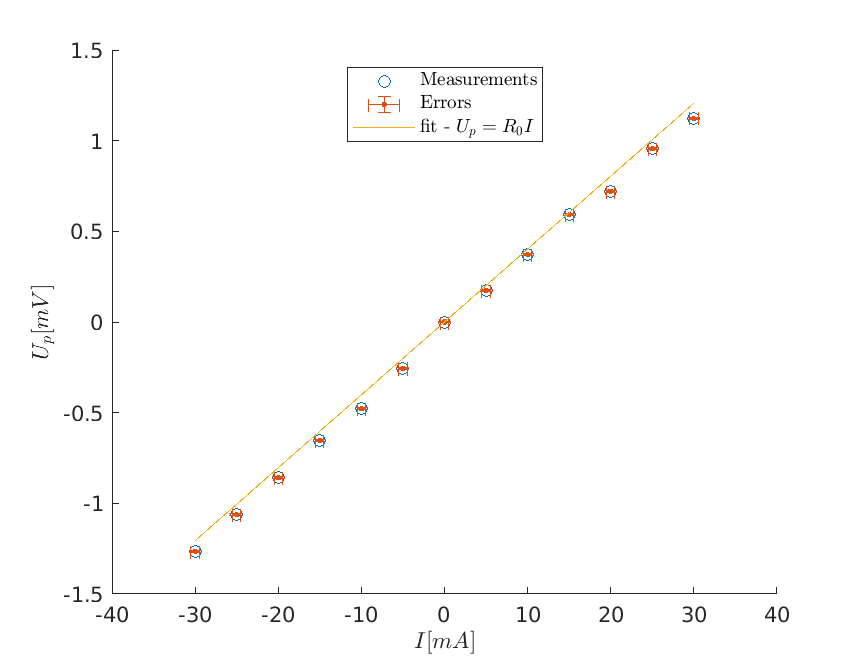
\includegraphics[width=0.8\textwidth]{part0 - R_0.png}
    \caption{Caption}
    \label{fig:part_0}
\end{figure}


לאחר מכן הפעלנו שדה מנגטי בניצב לכיוון הזרם בגודל של 
$B = (250 \pm 1) mT$ 
לשם קבלת אפקט הול. תוצאות מדידת מתח הול כתלות בזרם מוצגות בגרף
\ref{fig:part_1}.

\begin{figure}[ht!]
    \centering
    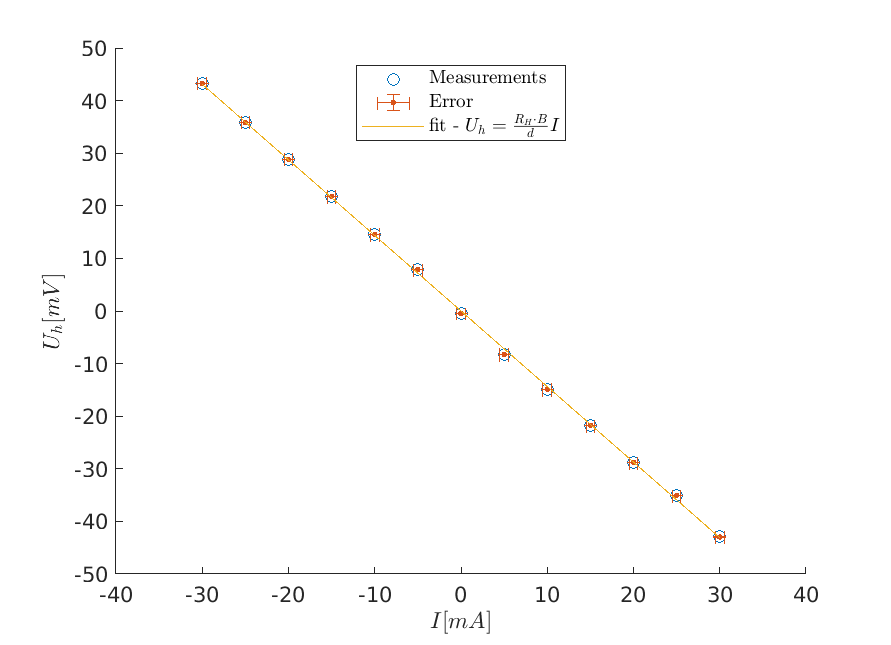
\includegraphics[width=0.8\textwidth]{part1 - R_h.png}
    \caption{Caption}
    \label{fig:part_1}
\end{figure}
לאחר מכן קבענו זרם קבוע של
$I = (30 \pm 1) mA$,
ושנינו את השדה המגנטי.
בגרף
\ref{fig:part_2}.
מוצגות מדידות של מתח הול כתלות בשדה המגנטי,
ובגרף
\ref{fig:part_3}.
מוצגות מדידות של המתח הישר כתלות בשדה המגנטי.

\begin{figure}[ht!]
    \centering
    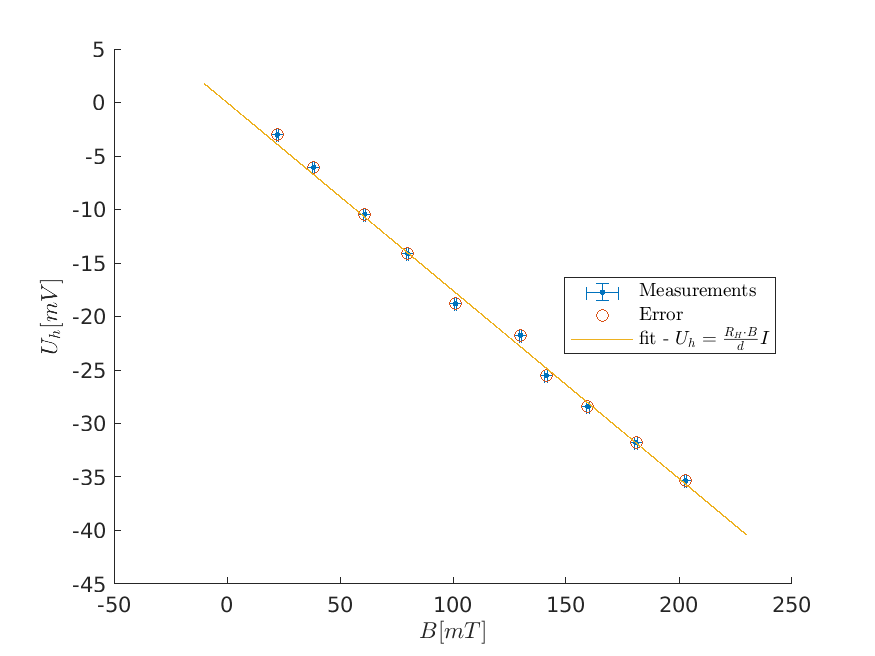
\includegraphics[width=0.8\textwidth]{part2 - R_h.png}
    \caption{Caption}
    \label{fig:part_2}
\end{figure}

\begin{figure}[ht!]
    \centering
    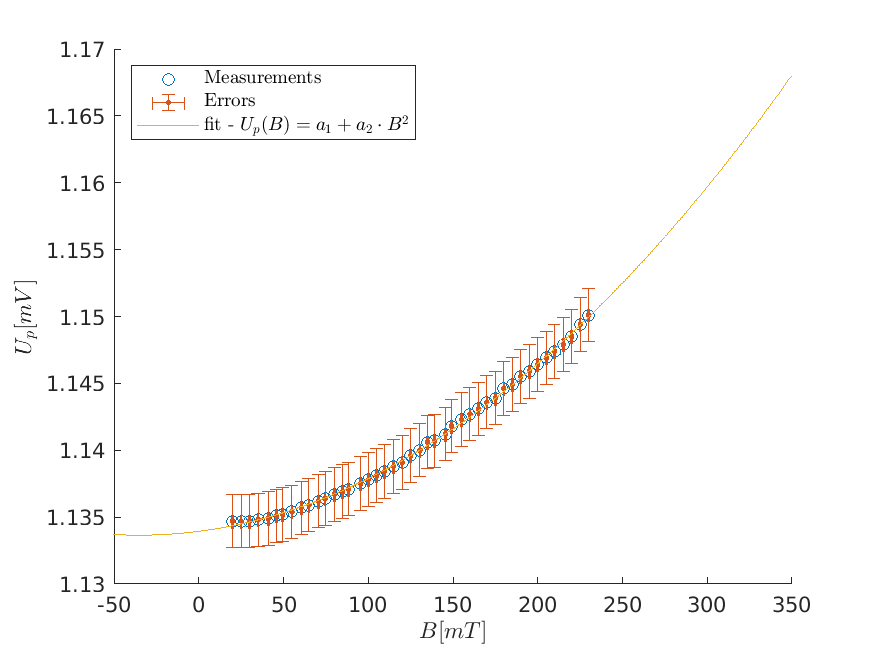
\includegraphics[width=0.8\textwidth]{part3 - B-squared relation}
    \caption{Caption}
    \label{fig:part_3}
\end{figure}
    
לבסוף מדדנו את הקשר בין מתח הול והמתח הישר לטמפרטורה,
התוצאות מוצגות בגרפים
\ref{fig:part_4}
ו-
\ref{fig:part_5}
בהתאמה.

\begin{figure}[ht!]
    \centering
    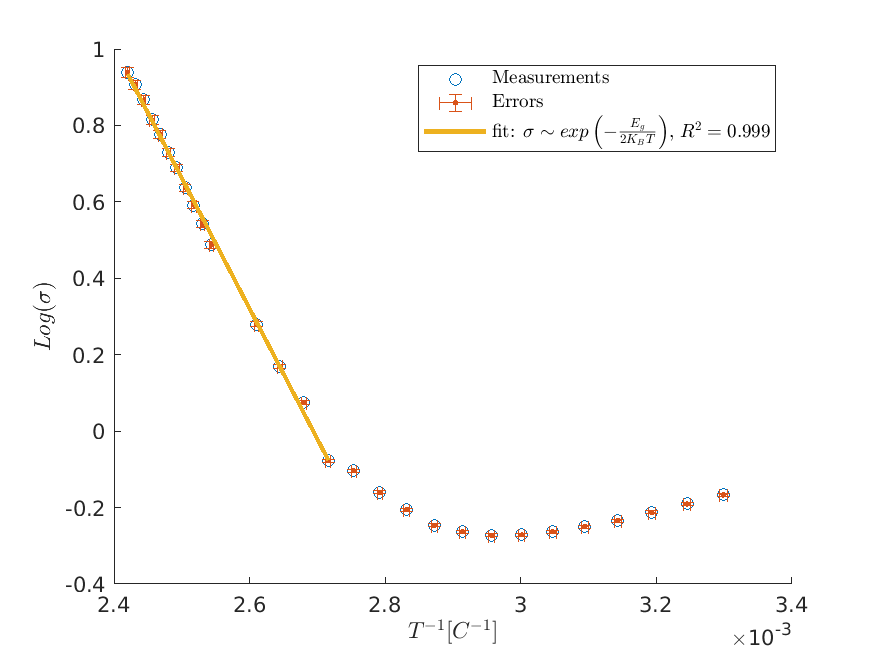
\includegraphics[width=0.8\textwidth]{part4 - E_g.png}
    \caption{Caption}
    \label{fig:part_2}
\end{figure}

\begin{figure}[ht!]
    \centering
    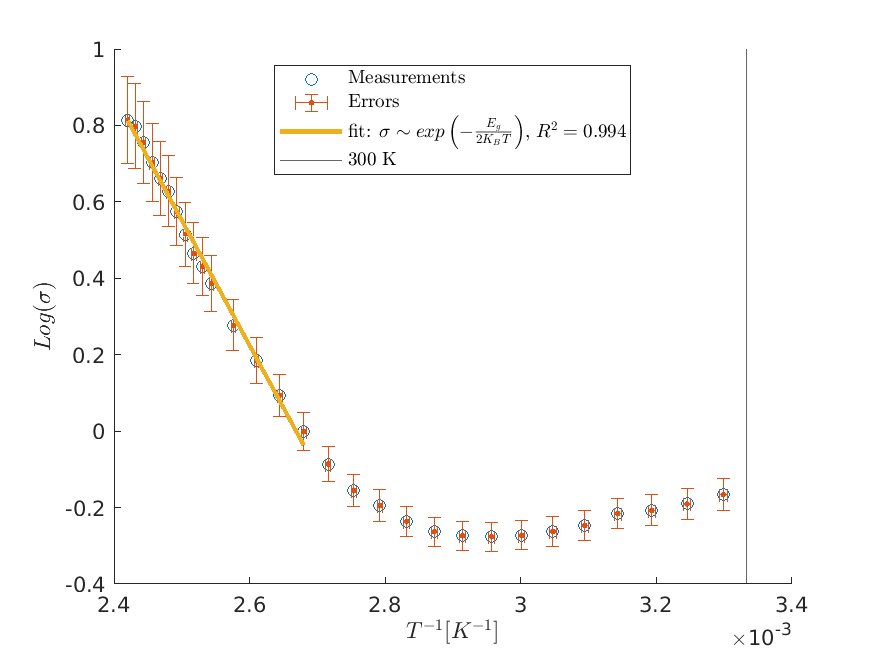
\includegraphics[width=0.8\textwidth]{part5 - E_g with magnetic field.png}
    \caption{Caption}
    \label{fig:part_3}
\end{figure}



\end{document}